\documentclass[tikz,border=2pt]{standalone}
\renewcommand{\familydefault}{\sfdefault}
\usetikzlibrary{arrows.meta,calc,positioning}
\tikzset{every picture/.style={line width=1pt, >=Stealth},
         hl/.style={fill=black, fill opacity=0.12, text opacity=1}}
\begin{document}
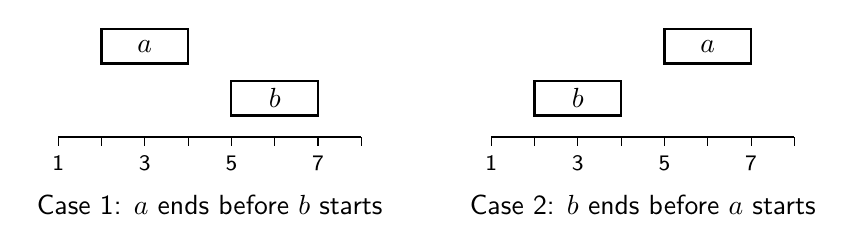
\begin{tikzpicture}[thick, x=0.55cm, y=0.55cm]
  \foreach \dx/\as/\ae/\bs/\be/\txt in {
      0/2/4/5/7/{Case 1: $a$ ends before $b$ starts},
      10/5/7/2/4/{Case 2: $b$ ends before $a$ starts}} {
    \begin{scope}[shift={(\dx,0)}]
      \draw[thin] (1,0) -- (8,0);
      \foreach \t in {1,...,8} \draw[thin] (\t,0) -- (\t,-0.2);
      \foreach \t in {1,3,5,7} \node[below, font=\footnotesize] at (\t,-0.2) {\t};
      \draw (\as,1.7) rectangle node {$a$} (\ae,2.5);
      \draw (\bs,0.5) rectangle node {$b$} (\be,1.3);
      \node[below] at (4.5,-1.1) {\txt};
    \end{scope}
  }
\end{tikzpicture}
\end{document}
